\documentclass{article}
\usepackage{color}
\usepackage{graphicx}

\begin{document}
\let\thefootnote\relax\footnotetext{Last edited January 17, 2015 by KO}

Summary of the data preprocessing:
\begin{itemize}
\item We split the data by year, 1990 and 2010, in which the sodium data was recorded. Within each of these datasets, we imputed the missing values for predictors by taking the median for that variable.
\item Sex-specific alcohol consumption measurements were only available in 2010, so we used overall alcohol consumption for 1990. No other predictor was sex-specific. 
\item We removed Chile from the analysis because there was no life expectancy data for 2010. 36 countries remained.
\item	We took the difference between 2010 and 1990 for all (numeric) variables.
\end{itemize}

We tested the hypothesis of association between sodium intake and excess mortality.  In our dataset, ``excess mortality'' is signified by a decrease in life expectancy from 1990 to 2010 beyond what would be expected given all other characteristics of a country.  We measured this by modeling the change in life expectancy using all the other available variables, including alcohol consumption, population, real GDP, and other economic and social variables.  For our dataset, we tried several predictive models and found that ordinary linear regression on all the variables gave the smallest within-sample mean square error.  The residuals from this model represent the change in life expectancy not explained by the measured variables. \\

We measured the strength of the association between sodium intake and the residuals from the model using Pearson's correlation. We tested the significance of the association using a permutation test.  Under the null hypothesis of no association, the residuals of the model are exchangeable: if sodium intake has no effect on mortality, then the residuals are equally likely to be paired with any of the sodium measurements.  Under the alternative hypothesis, our model will tend to \textit{overestimate} the increase in life expectancy from 1990 to 2010 in countries where sodium intake increased and to \textit{underestimate} the change in life expectancy in countries where sodium intake decreased. This alternative corresponds to a significant positive correlation between the residuals and change in sodium intake.  The correlation for males was $-0.1288$ (one-sided p-value $0.7796$, two-sided p-value $0.4471$) and the correlation for females was $-0.08257$ (one-sided p-value $0.6857$, two-sided p-value $0.6298$). We conclude there is insufficient evidence to reject the null hypothesis that the correlation is $0$. \\

We obtained approximate confidence intervals for the estimates by inverting the permutation test.  The endpoints were computed by shifting the entire permutation distribution up to the smallest amount for which we would reject the null hypothesis. (still unsure of the justification for this) The two-sided $95\%$ confidence interval for the correlation for males was $(-0.5888, 0.0862)$ and for females was $(-0.4976, 0.1774)$.


\begin{figure}
\centering
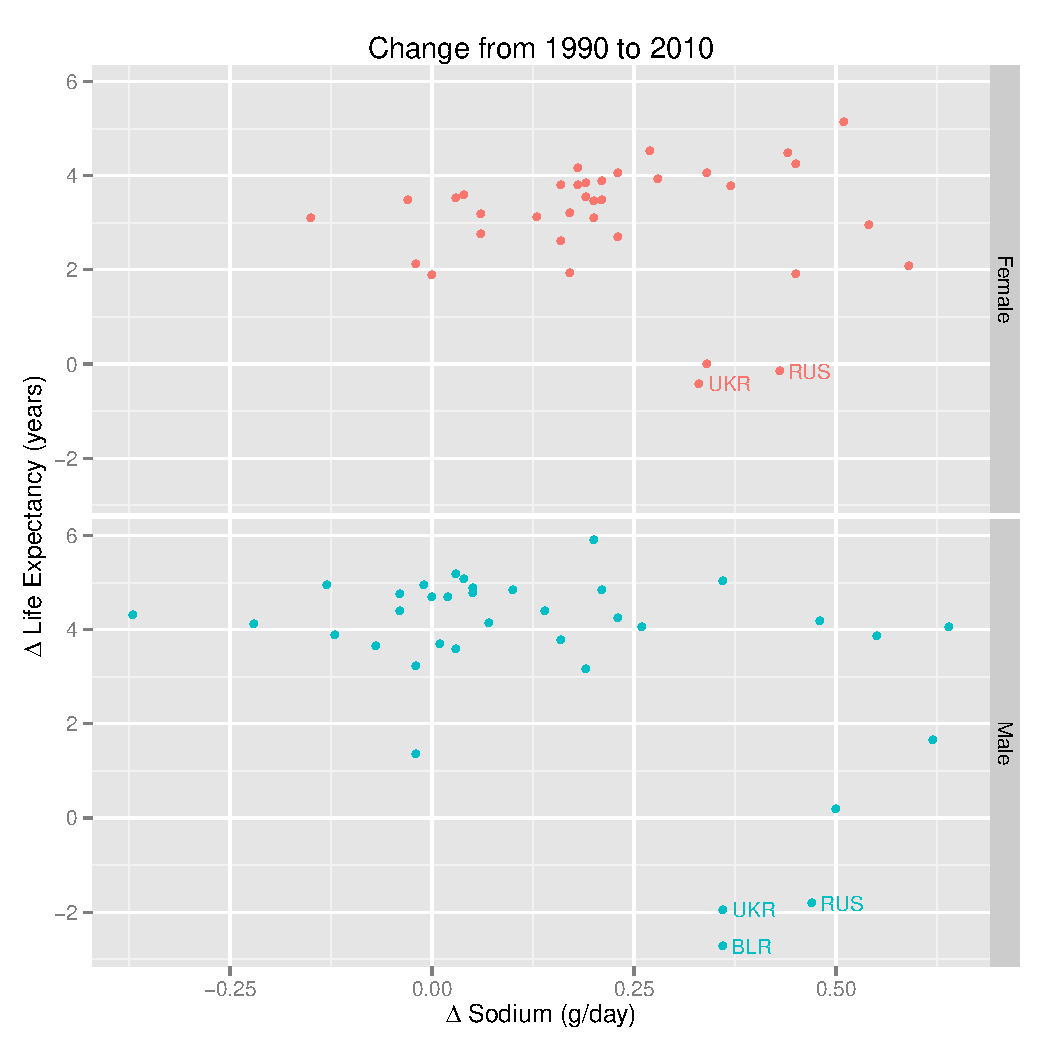
\includegraphics[width = \textwidth]{sodium_lifeexp.pdf}
\caption{Scatterplot of change in sodium intake against change in life expectancy at age 30 from 1990 to 2010. Even before correcting for the effect of other social and economic factors, there is no obvious association between sodium and life expectancy.}
\end{figure}
\begin{figure}
\centering
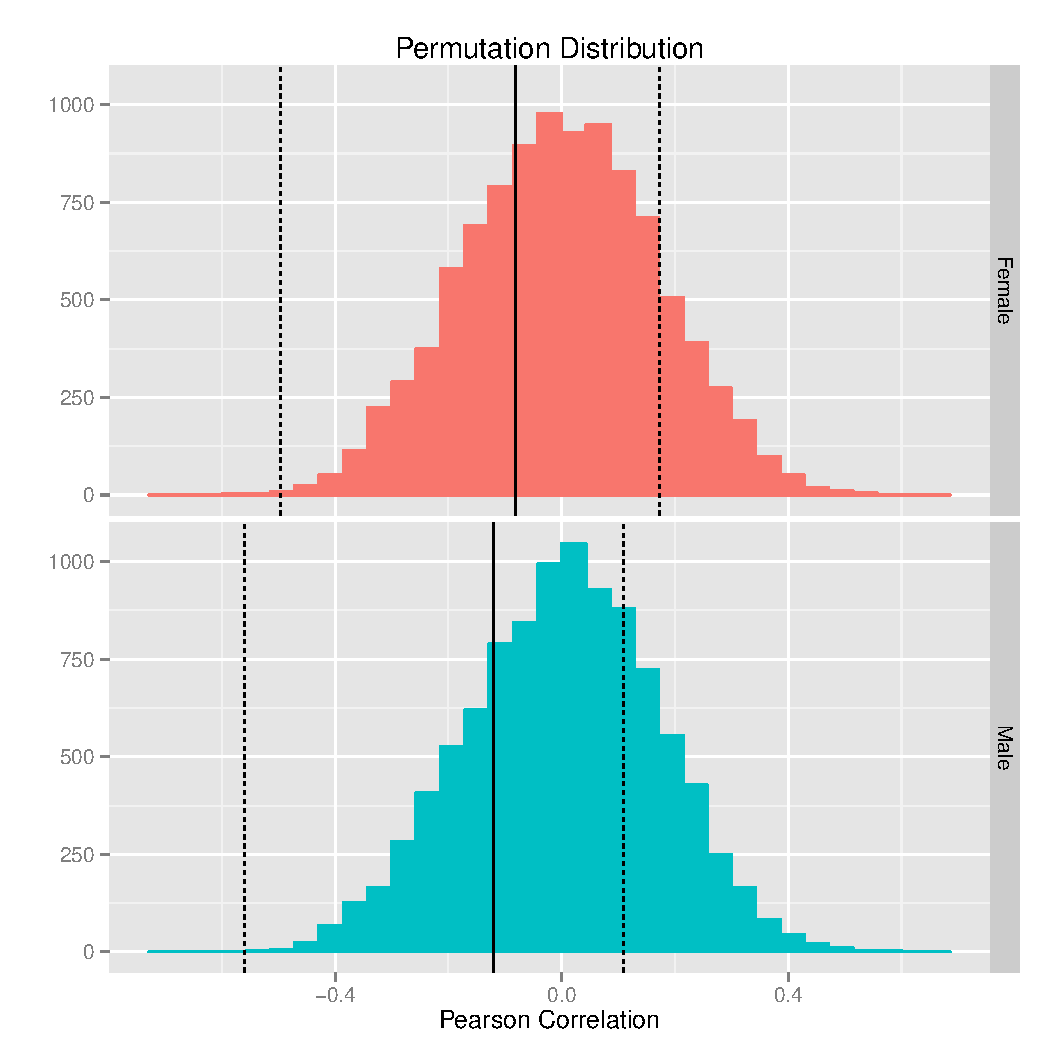
\includegraphics[width = \textwidth]{permdistribution.pdf}
\caption{Permutation distribution of Pearson correlation between change in sodium intake and the residuals from the model predicting change in life expectancy from all other variables. The solid line is the estimated correlation and the dotted lines are the confidence interval endpoints.}
\end{figure}

\end{document}